In this chapter the function test of the final robot will be described. In relation to the specified requirements in \secref{sec:requirement_specification}, all the requirements is tested. The tests show whether or not the robot is able to perform the actions from the requirements. It is not possible to test the physical features but they have been fulfilled.

The requirements for the robot: 
\begin{itemize}
\item Navigate the environment within the boundaries.
\item Control collection arm to pick up and store objects of specified size.
\item Find and collect all objects within the time limit.
\end{itemize}


\section{Test setup}
To test the \projname{} and its ability to fulfil the three requirements, a testing area similar to a real world environment was set up. This area was determined by a boundary, which the robot was not allowed to cross, and a certain amount of objects with a size and weight that the robot earlier have proven to be able to find and collect, see \secref{sec:object_specification} for details about what objects that can be collected.

\begin{figure}[H]
     \center\frame{{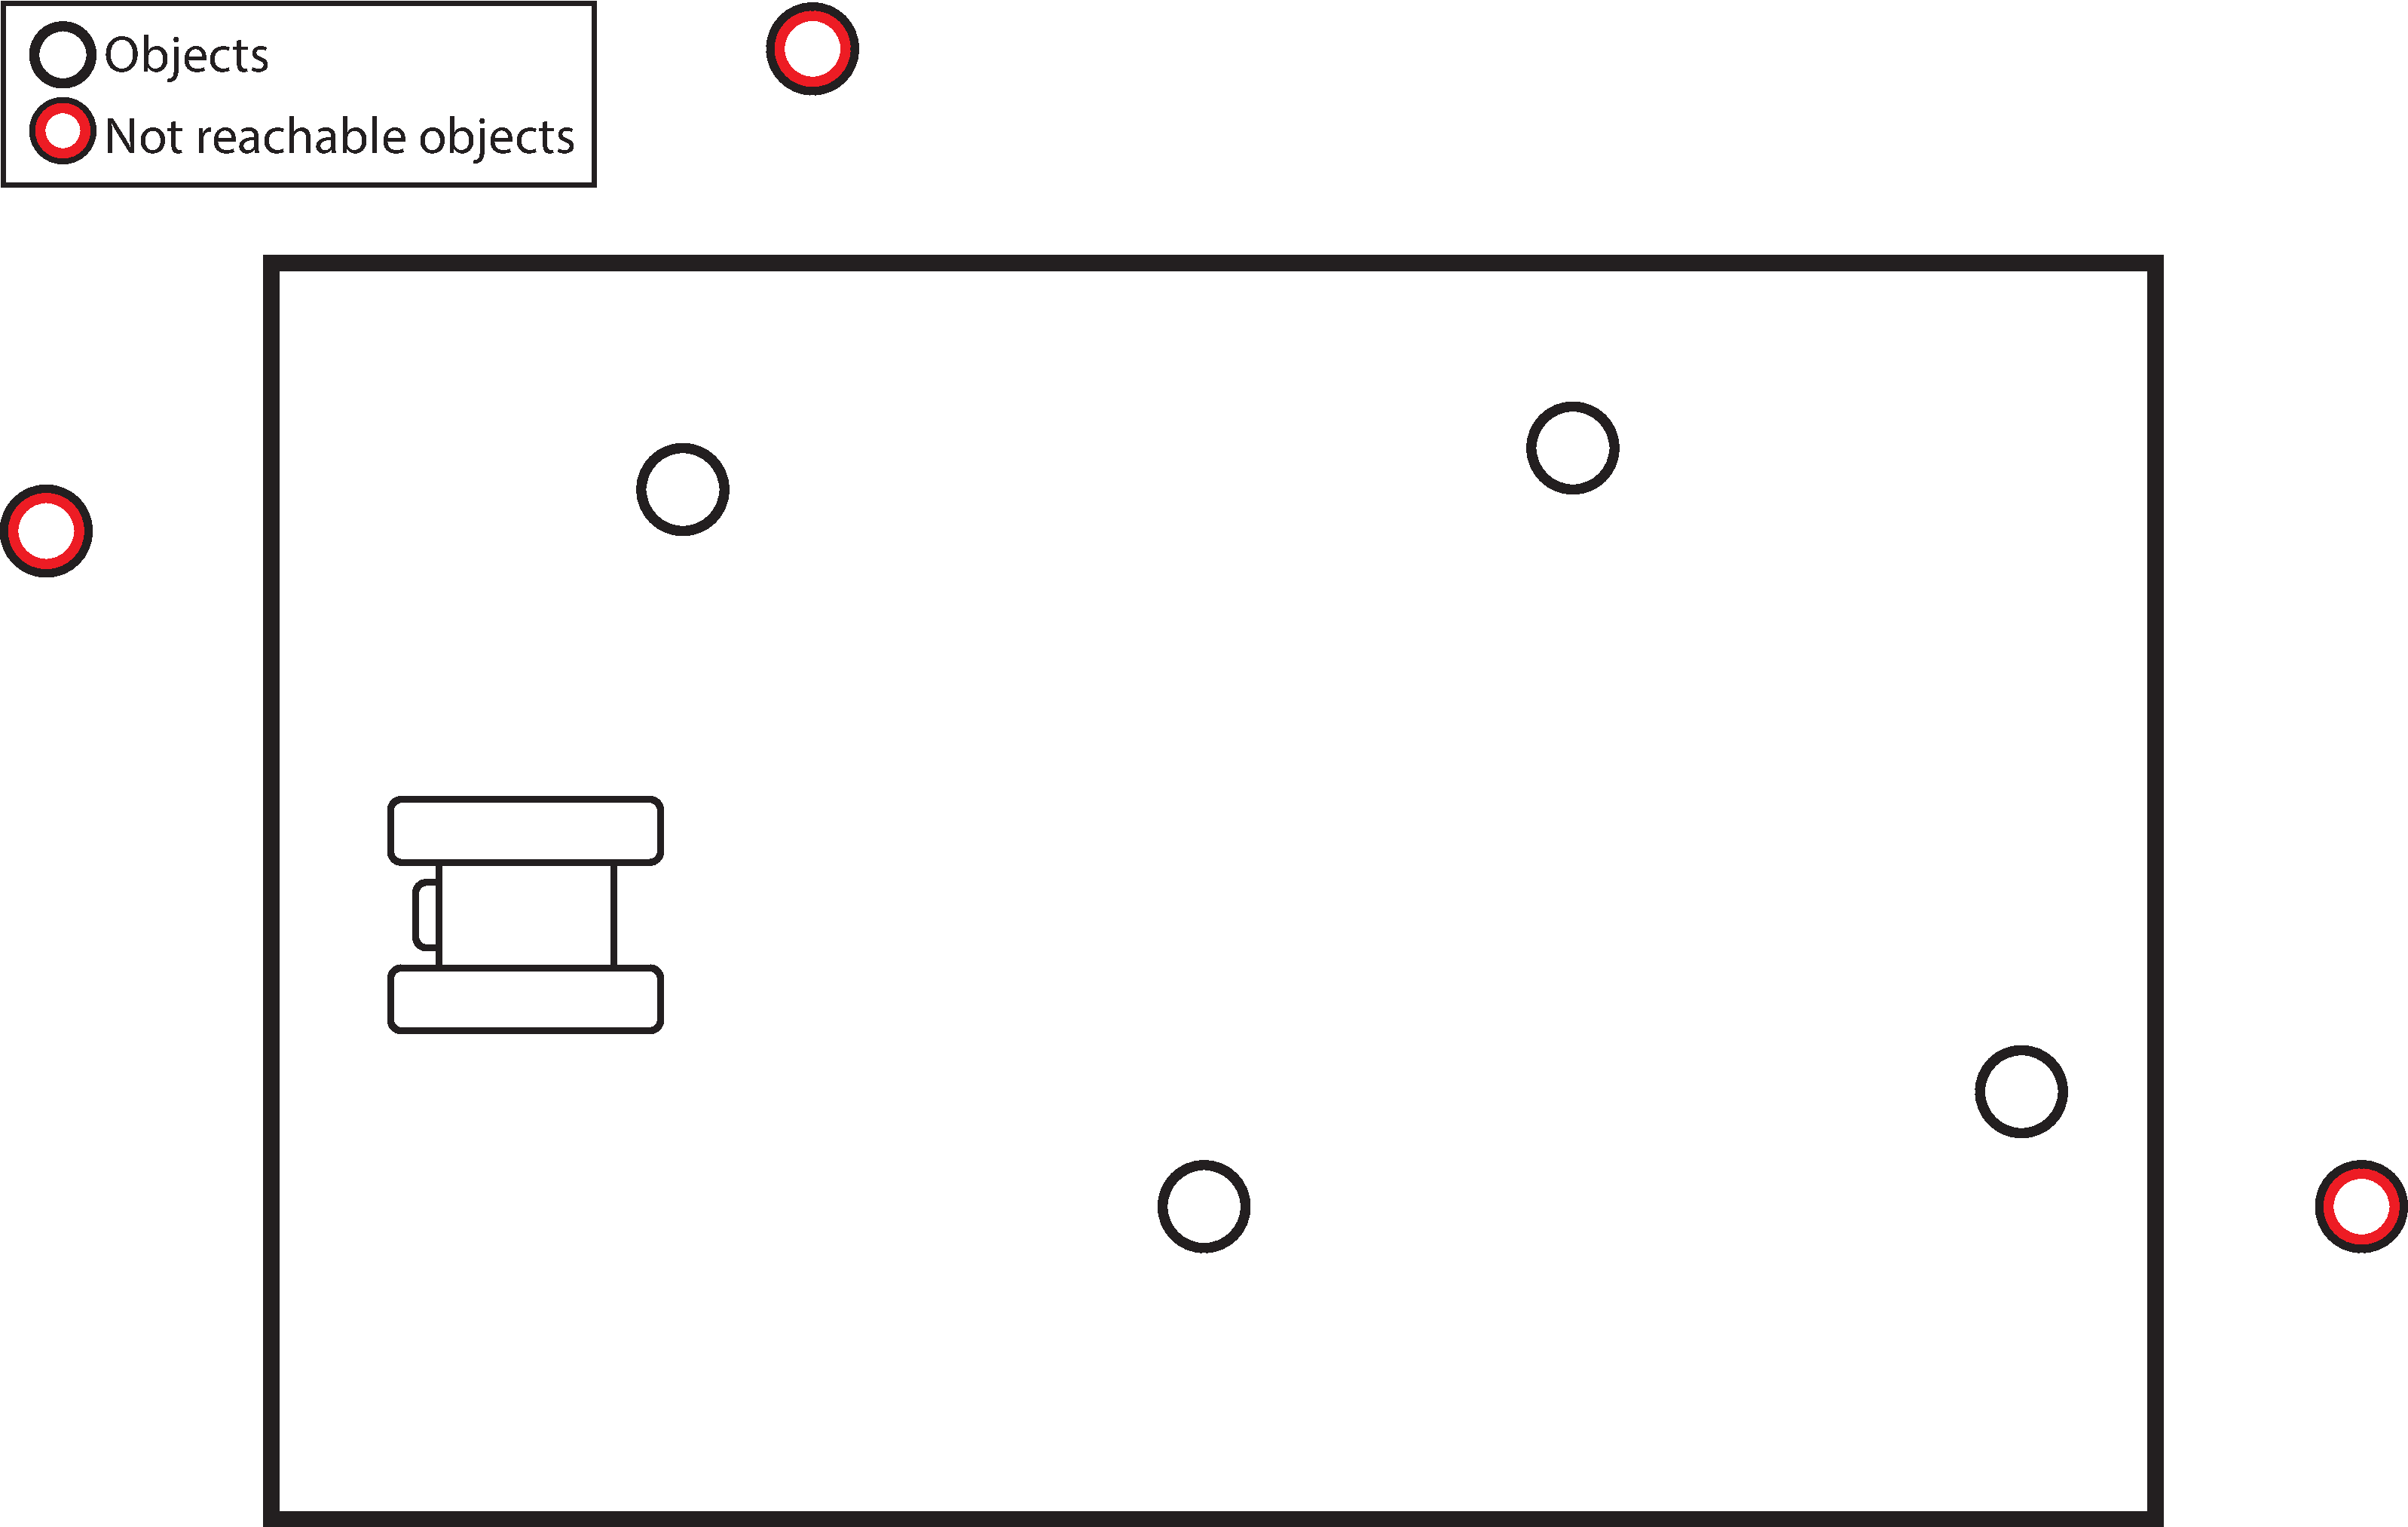
\includegraphics[width=320pt]
     {graphics/TestSetup.pdf}}}
     \caption{\label{fig:test-setup} Example of a tested environment.}
\end{figure}

The area was a rectangle with the dimensions 1 m times 1.5 m framed by double layer of black tape. Each test included four cans used as objects. Each can had were 7 cm high, had a diameter of 6.5 cm, and weighted 10 g. An example of a tested environment can be seen in \figref{fig:test-setup}

\section{Test result}

All the requirements was tested in one combined test but for each requirement there is made some observations. The observations for all three requirements is listed below.

\textbf{Navigate the environment within the boundaries}
\begin{itemize}
\item Sometimes the robot not detects the black lines before its too late.
\item The width of the black lines is important. If the black line is to thin the robot will often not detect the lines.
\end{itemize}

\textbf{Control collection arm to pick up and store objects of specified size}
\begin{itemize}
\item The signal form the slave to the master is not always received when it is finished.
\item Sometimes the robot not see a object even if it is right in the front of the robot.
\end{itemize}
\textbf{Find and collect all objects within the time limit}
\begin{itemize}
\item If the distance between the objects is too big, the robot will never find all the object. 
\item The time used to find objects increases if there is objects on the other side of the black lines.  
\end{itemize}

In addition to the observations the \tblref{table:FinalTimeTestRobot} shows the time result from the test. The time result is acceptable i relation to the goal from \secref{sec:model}.

\begin{table}[H]
	\centering
	\ra{1.3}
  \rowcolors{1}{Gray}{}
   \begin{tabular}{|c|c|c|c|}
   \hline  
   Test no. & Time & Objects & Average time pr. object \\ \hline
      1    & 98.0 seconds    & 4 & 24.5 seconds   \\ \hline
      2    & 98.0 seconds    & 4 & 24.5 seconds  \\ \hline
      3    & 99.0 seconds    & 4 & 24.8 seconds  \\ \hline
      4    & 87.0 seconds    & 4 & 21.8 seconds  \\ \hline
      5    & 108.0 seconds   & 4 & 27.0 seconds  \\ \hline
   \end{tabular}
   \caption{\label{table:FinalTimeTestRobot} Time test of the robot}
\end{table}







